\documentclass[aspectratio=169]{beamer}
\mode<presentation>
%\usetheme{Warsaw}
%\usetheme{Goettingen}
\usetheme{Hannover}
%\useoutertheme{default}

%\useoutertheme{infolines}
\useoutertheme{sidebar}
\usecolortheme{dolphin}

\usepackage{amsmath}
\usepackage{amssymb}
\usepackage{enumerate}

%some bold math symbols
\newcommand{\Cov}{\mathrm{Cov}}
\newcommand{\Cor}{\mathrm{Cor}}
\newcommand{\Var}{\mathrm{Var}}
\newcommand{\brho}{\boldsymbol{\rho}}
\newcommand{\bSigma}{\boldsymbol{\Sigma}}
\newcommand{\btheta}{\boldsymbol{\theta}}
\newcommand{\bbeta}{\boldsymbol{\beta}}
\newcommand{\bmu}{\boldsymbol{\mu}}
\newcommand{\bW}{\mathbf{W}}
\newcommand{\one}{\mathbf{1}}
\newcommand{\bH}{\mathbf{H}}
\newcommand{\by}{\mathbf{y}}
\newcommand{\bolde}{\mathbf{e}}
\newcommand{\bx}{\mathbf{x}}

\newcommand{\cpp}[1]{\texttt{#1}}

\title{Mathematical Biostatistics Boot Camp 2: Lecture 3, Two Sample Tests}
\author{Brian Caffo}
\date{\today}
\institute[Department of Biostatistics]{
  Department of Biostatistics \\
  Johns Hopkins Bloomberg School of Public Health\\
  Johns Hopkins University
}


%\logo{\includegraphics[height=0.5cm]{Logo_PPT.pdf}}

\begin{document}
\frame{\titlepage}

%\section{Table of contents}
\frame{
  \frametitle{Table of contents}
  \tableofcontents
}

\section{Matched data}
\begin{frame}\frametitle{Hypothesis testing for comparing two means}
\begin{itemize}
\item When comparing groups, first determine whether observations are
  paired or not
\item When dealing a single set of paired data, one strategy is to
  take the difference between the paired observation and do a
  one-sample $t$ test of $H_0:\mu_d = 0$ versus $H_a:\mu_d \neq 0$ (or
  one of the other two alternatives)
\item Test statistic is
  $$
  \frac{\bar X_d - \mu_{d0}}{S_d / \sqrt{n_d}}
  $$
  where $\mu_{d0}$ is the value under the null hypothesis (typically
  $0$); compare this statistic to a $t_{n_d -1}$ or $z$ statistic
\end{itemize}
\end{frame}

\begin{frame}[fragile]\frametitle{Example}
  \begin{itemize}
    \item Consider Exam 1 and Exam 2 grades from a previous class
    \item Is there any evidence that the second exam was easier or
      harder than the first?
    \item The same students took both exams with none dropping out in-between
    \item Summaries for the two exams
\begin{verbatim}
> summary(test1)
 Min. 1st Qu.  Median    Mean 3rd Qu.    Max.    
76.19   82.86   86.67   86.94   91.43  100.00     
> summary(test2)                
 Min. 1st Qu.  Median    Mean 3rd Qu.    Max.     
71.00   87.00   90.00   89.82   93.00  100.00    
\end{verbatim}
  \end{itemize}
\end{frame}


\begin{frame}
\begin{center}
  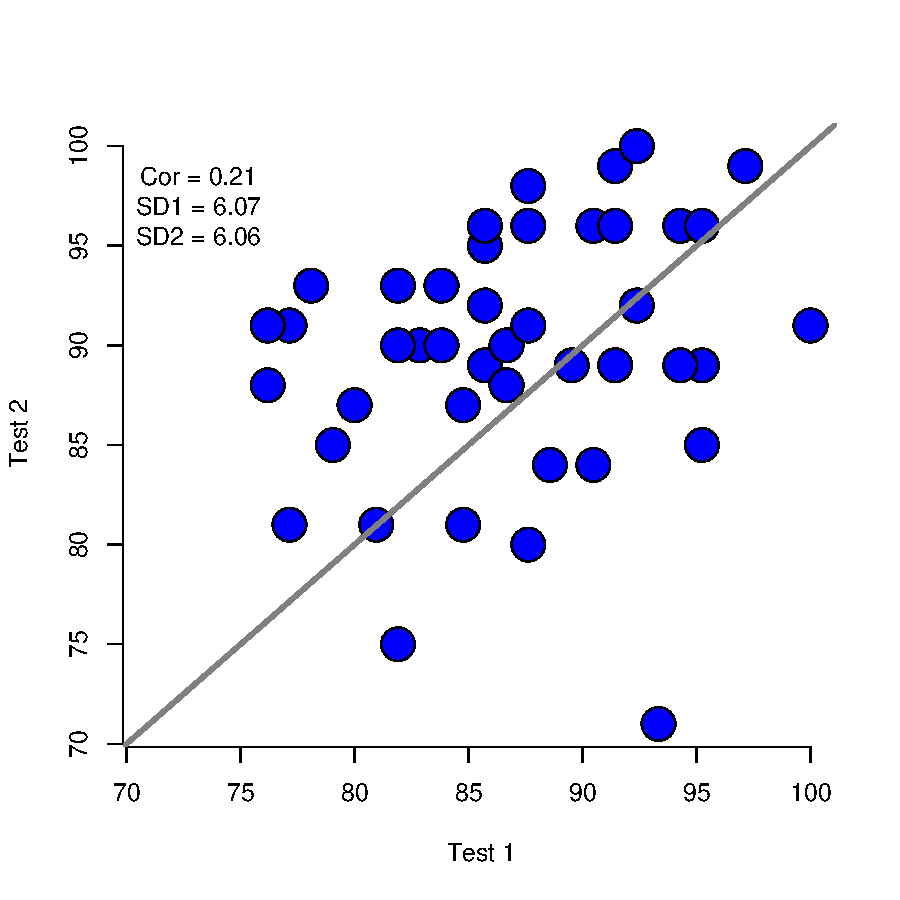
\includegraphics[height=3in]{pairPlot.pdf}
\end{center}
\end{frame}

\begin{frame}
\begin{center}
  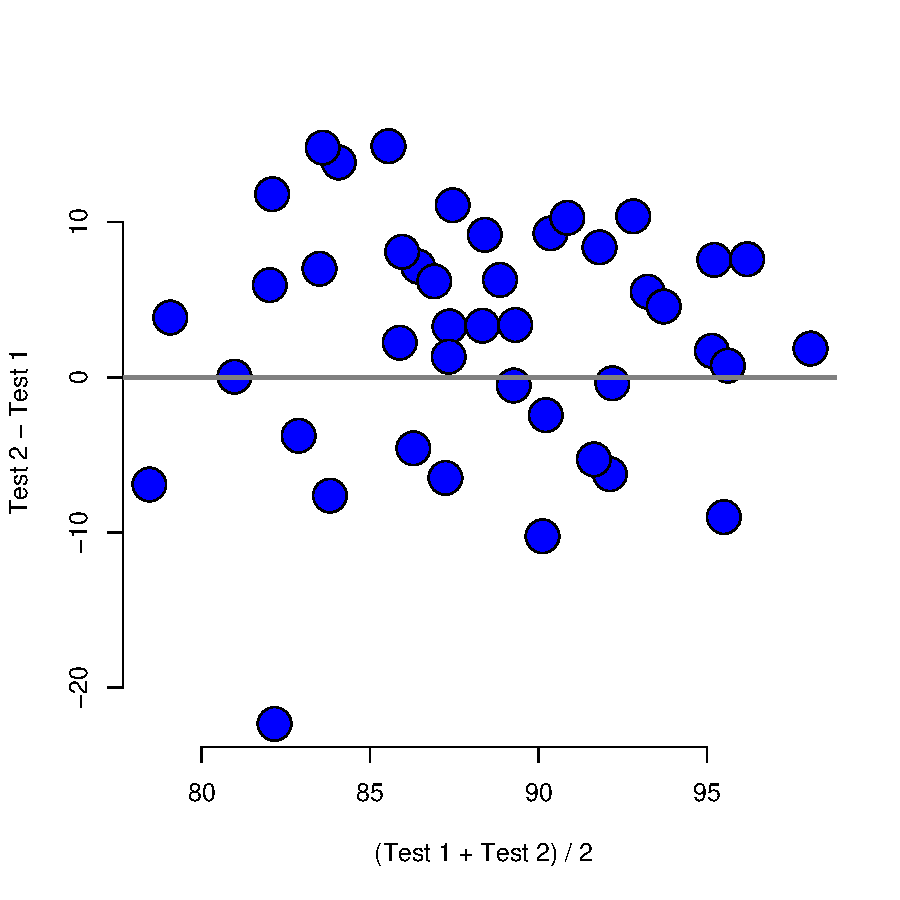
\includegraphics[height=3in]{tmd.pdf}
\end{center}
\end{frame}

\begin{frame}[fragile]
R Code
\begin{verbatim}
diff <- test2 - test1
n <- sum(!is.na(diff)) #49
mean(diff) #2.88
sd(diff) #7.61
testStat <- sqrt(n) * mean(diff) / sd(diff) #2.65
# below works out to be 0.01
2 * pt(abs(testStat), n -1, lower.tail = FALSE) 
##uses the R function
t.test(diff)
\end{verbatim}  
\end{frame}

\begin{frame}\frametitle{Discussion of matched data}
  \begin{itemize}
  \item Also to consider, ``are ratios more relevant than pair-wise
    differences?''; if so, try doing the test on the log-observations
  \item When considering matched pairs data, you often want to plot the first observation by the second
  \item A more efficient plot displays the average of the observations by the difference or doing this on the log scale
  \item The previous plot is called a ``mean/difference'' plot,
    invented by Tukey (sometimes it is called a ``Bland/Altman'' plot
    after researchers who effectively described and used the method
    for considering measurement error)
  \end{itemize}
\end{frame}

\section{Aside,  regression to the mean}
\begin{frame} \frametitle{Regression to mediocrity}
  \begin{itemize}
  \item Francis Galton was the first to recognize that for matched
    data, high initial observations tended to be associated with lower
    second observations and low initial observations tended to be
    associated with higher second observations
  \item Example: Sons of very tall fathers tend to be a little shorter
    (also fathers of very tall sons tend to be shorter)
  \item Example: Second exams for those who scored very high on a
    first exam tend to be a little lower
  \end{itemize}
\end{frame}

\begin{frame}
  \begin{center}
    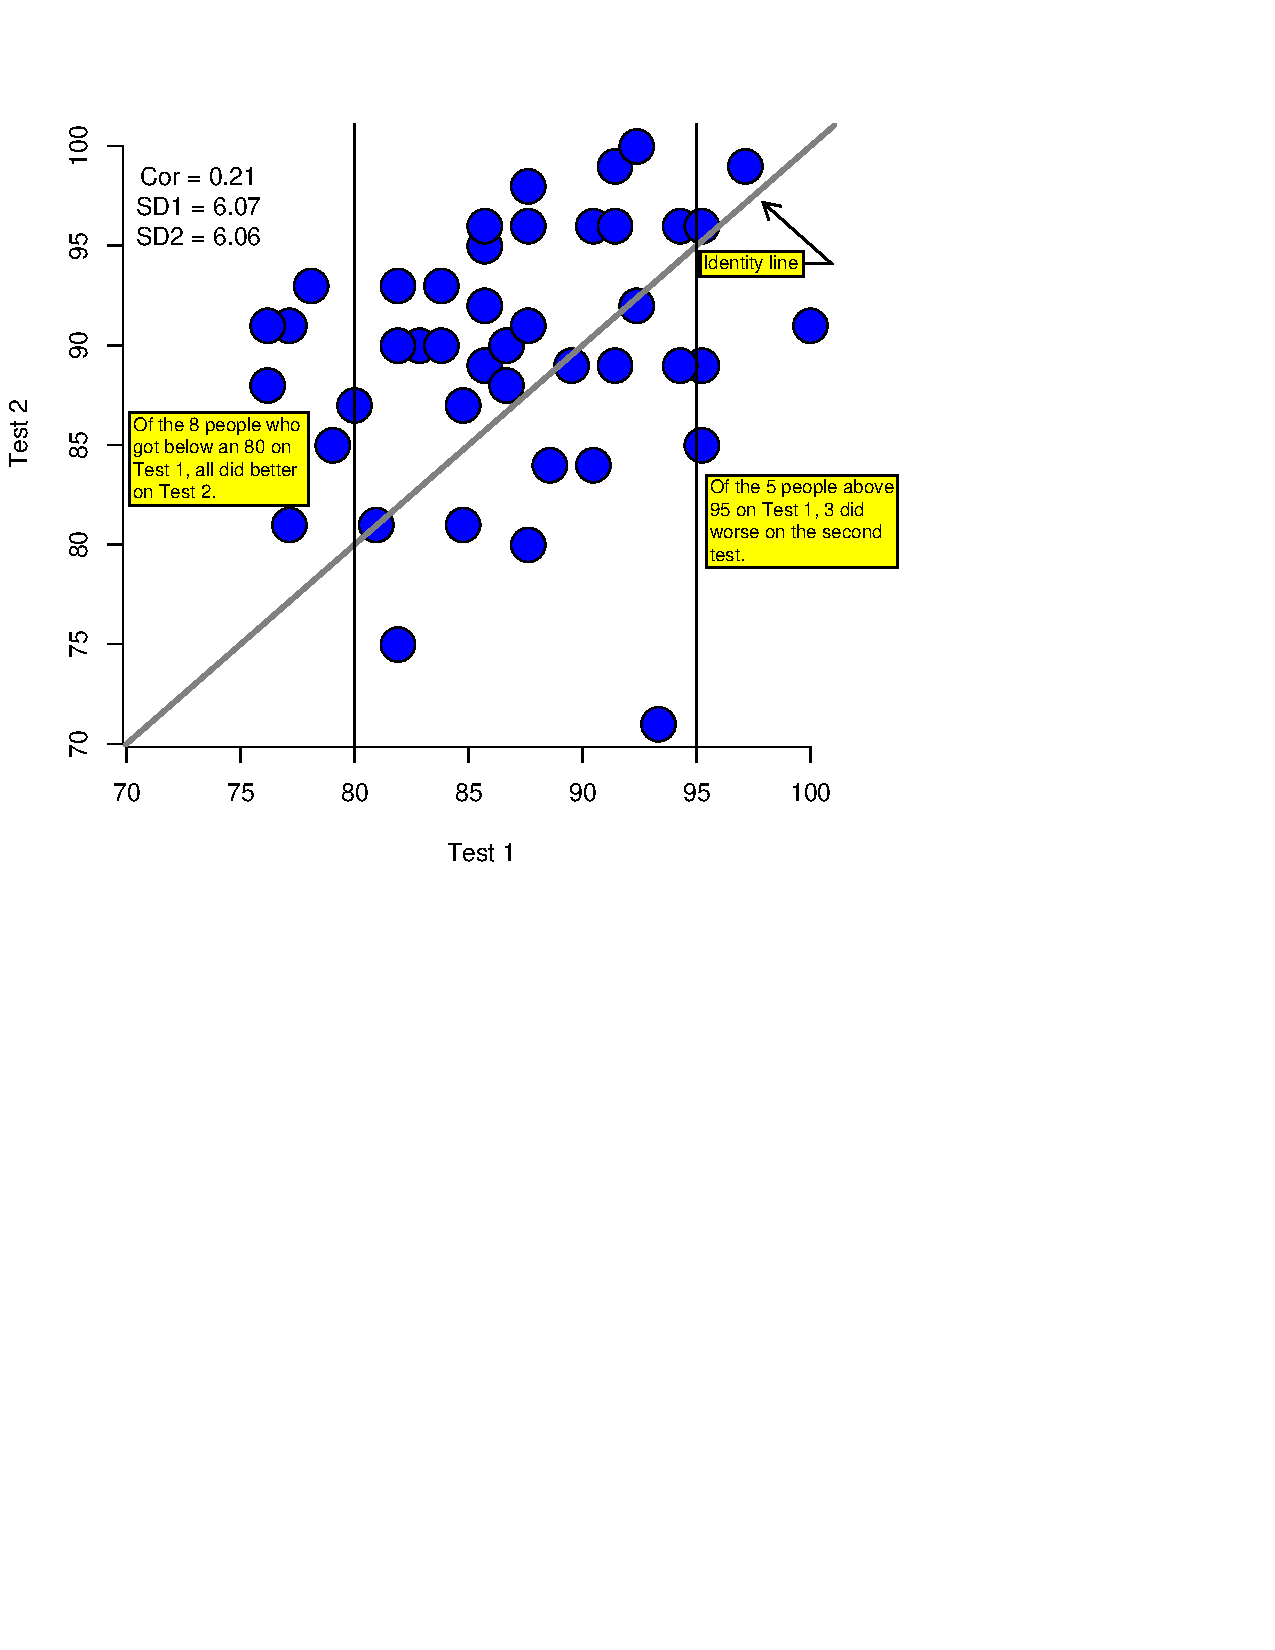
\includegraphics[height=3in]{rtmAnotated.pdf}
  \end{center}
\end{frame}

\begin{frame}\frametitle{RTM continued}
  \begin{itemize}
     \item To investigate more, we normalize both scales (so that their
       means are both 0 and standard deviations 1)
     \item If there was no regression to the mean, the data would
       scatter about an identity line
     \item The best fitting line goes through the average and has slope 
       $$\Cor(Test1, Test2) \frac{\mathrm{SD}(Test2)}{\mathrm{SD}(Test1)}$$
       and passes 
       through the point $$\{\mathrm{mean}(Test1),\mathrm{mean}(Test 2)\}$$.
     \item Because we normalized the data, our line passes through $(0, 0)$ and 
       has slope $\Cor(Test1, Test2)$ (normalizing doesn't impact the correlation)
  \end{itemize}
\end{frame}

\begin{frame}\frametitle{RTM continued}
  \begin{itemize}
    \item The best fitting ``regression line'' has slope $\Cor(Test1, Test2)<1$
    \item This will be shrunk toward a horizontal line, telling us our
      expected normalized test score for Test 2 will be $\Cor(Test1, Test2)$
      times the normalized Test 1 score
    \item This line appropriately adjusts for regression to the mean for
      Test 2 conditioning on Test 1; we could similarly do the same for
      Test 1 conditioning on Test 2; this line will have slope $\Cor(Test1, Test2)^{-1}$
      if plot with Test 1 on the horizontal axis
    \item The latter line will be shrunk toward a vertical line; the
      identity line will fall between the two
  \end{itemize}
\end{frame}

\begin{frame}
  \begin{center}
    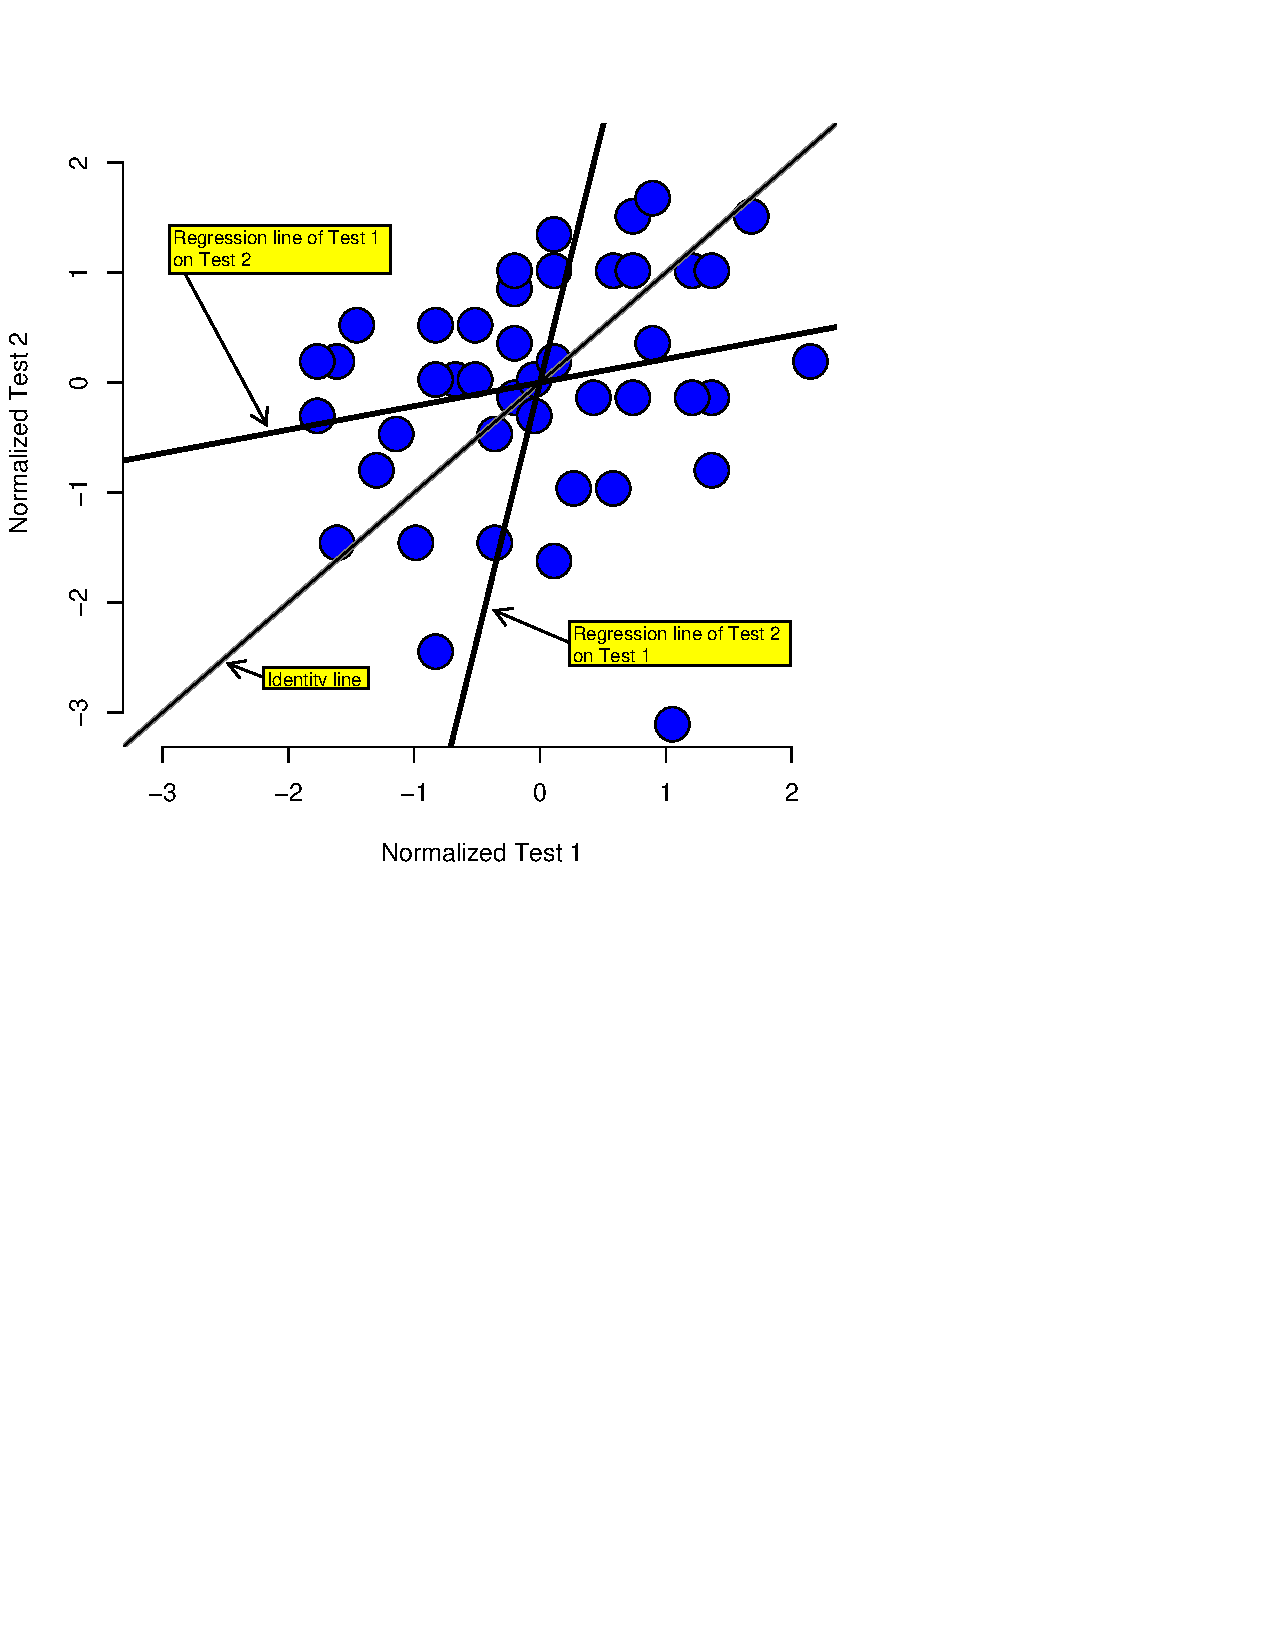
\includegraphics[height=3in]{rtm2Anotated.pdf}    
  \end{center}
\end{frame}

\begin{frame}\frametitle{Final comments}
  \begin{itemize}
     \item An ideal examiner would have little difference between the identity line
       and the fitted regression line
     \item The more unrelated the two exam scores are, the more pronounced the regression to the mean
     \item If you watch sports you have to wonder how much discussion
       is over regression to the mean
     \item Athletes who perform the best will often perform worse the
       next year; is this regression to the mean or an actual decline
       in the athlete's ability?
  \end{itemize}
  
\end{frame}

\section{Two independent groups}
\begin{frame}\frametitle{Two independent groups}
\begin{itemize}
\item The extension to two independent groups should come as no surprise
\item $H_0:\mu_1 = \mu_2$, versus $H_a:\mu_1 \neq \mu_2$ (or one of the other
  two alternatives)
\item Assuming a common error variance we have
  $$
  \frac{\bar X - \bar Y}{S_p \sqrt{\frac{1}{n_x} +
      \frac{1}{n_y}}}
  $$
  which will follow a $t_{n_x + n_y - 2}$ distribution under the null
  hypothesis and the usual assumptions
\end{itemize}
\end{frame}

\begin{frame}\frametitle{Continued}
\begin{itemize}
\item If the assuming a common error variance is questionable
$$
  \frac{\bar X - \bar Y}{\sqrt{\frac{S_x^2}{n_x} + \frac{S_y^2}{n_y}}}
  $$
  follows a standard normal distribution for large $n_x$ and $n_y$.
  It follows an approximate Students $T$ distribution if the $X_i$ and
  $Y_i$ are normally distributed 
\item The approximate degrees of freedom are
  $$
  \frac{(S_x^2 / n_x + S_y^2 / n_y)^2}{(S_x^2 / n_x)^2 / (n_x - 1) + (S_y^2 / n_y)^2 / (n_y - 1)}
  $$
\end{itemize}
\end{frame}

\begin{frame}
\begin{itemize}
\item Note the connection between hypothesis testing and confidence
  intervals still holds; for example, if zero is in your independent 
  group $T$ interval, you will fail to reject the independent group $T$
  test for equal means
\item Don't test for equality of means by comparing separately
  constructed intervals for the two groups and rejecting the null
  hypothesis if they do not overlap
\item This procedure has lower power than just doing the right test
\item Also, it leads to the potential abuse of comparing intervals for
  paired data
\end{itemize}
\end{frame}

\begin{frame}\frametitle{Example}
  \begin{itemize}
     \item Suppose that instead of having repeated data on two consecutive exams,
       students were randomized to two teaching modules and took the same exam
     \item We might obtain data like the following
       \begin{center}
       \begin{tabular}{lllll}
         Group    & N  & Mean Exam & SD Exam \\
         Module 1 & 50 & 86.9 & 6.07 \\
         Module 2 & 50 & 89.8 & 6.06 \\ 
      \end{tabular}         
       \end{center}
     \item Pooled standard deviation $6.065$\footnote{note this is not obtained by averaging the two standard deviations, it's obtained by averaging the variances then square rooting}
     \item Test stat $$\frac{89.8 - 86.9}{6.065\sqrt{\frac{1}{50}+\frac{1}{50}}}$$
       (you do the rest)
  \end{itemize}
\end{frame}

\begin{frame}
\begin{itemize}
\item Look over the review notes on formal tests for equality of
  variances between two groups
\item These tests, employing the $F$ distribution, rely heavily on 
  normality assumptions
\item Alternatively, for moderate sample sizes, consider creating a
  bootstrap confidence interval for the ratio of the two variances
\item For smaller sample sizes, consider basing decisions on exploratory
  data analysis
\end{itemize}
\end{frame}

\begin{frame}\frametitle{Final comments}
  \begin{itemize}
    \item Suppose you have equal numbers of observations for two groups (say $X$ and $Y$)
    \item If the data are truly matched, then the standard error of the
      difference is estimating
      $$
      \sqrt{\frac{\sigma_y^2}{n} + \frac{\sigma_x^2}{n} - 2 \frac{\Cov(X, Y)}{n}}
      $$
    \item If you ignore the matching, then the standard
      error of the difference is estimating
      $$
      \sqrt{\frac{\sigma_y^2}{n} + \frac{\sigma_x^2}{n}}
      $$
    \item Since, generally, matched data is positively correlated, by
      ignoring the matching you are likely (violating assumptions and)
      inflating your standard error unnecessarily
  \end{itemize}
  
\end{frame}

\end{document}

